\newpage

\section{Results}

\subsection{Grid Convergence Without an Exact Solution}
\label{subsec:apf_grid_convergence}

Since an exact solution for the complete temperature field is
unavailable, spatial convergence is assessed by comparing
solutions on three successively refined grids. Each solution
must satisfy the steady-state residual tolerance before the
grid-to-grid differences are evaluated.

The grid levels used are
\begin{equation}
M_1=(25,10),\qquad
M_2=(50,20),\qquad
M_3=(100,40),
\end{equation}
where each pair denotes the number of cells in the streamwise
and wall-normal directions. Both grid dimensions are doubled
at each refinement, giving a refinement ratio of two.

\subsubsection{Successive-Grid Differences}

Because the solutions are cell-centred and defined on different
grids, each fine-grid solution is restricted to its corresponding
coarser grid by averaging each $2\times2$ block:
\begin{equation}
T^{f\rightarrow c}_{ij}
=
\frac{1}{4}
\sum_{r=0}^{1}\sum_{s=0}^{1}
T^f_{2i+r,\,2j+s},
\label{eq:apf_grid_restriction}
\end{equation}
where the indices refer to the physical-cell arrays using
zero-based indexing.

The RMS difference between successive solutions is then
\begin{equation}
D_{k,k+1}
=
\sqrt{
\frac{1}{n_xn_y}
\sum_{i=1}^{n_x}\sum_{j=1}^{n_y}
\left(
T^{M_k}_{ij}
-
T^{M_{k+1}\rightarrow M_k}_{ij}
\right)^2
}.
\label{eq:apf_grid_difference}
\end{equation}

\begin{algorithm}[H]
\caption{APF Grid Self-Convergence Analysis}
\label{alg:apf_grid_self_convergence}
\begin{algorithmic}[1]
\Require Grid levels $M_1=(25,10)$, $M_2=(50,20)$,
$M_3=(100,40)$; residual tolerance $\varepsilon$;
pseudo-time step $\Delta t$
\Ensure Successive-grid differences $D_{12},D_{23}$,
observed order, fitted order, and convergence diagnostics

\State Initialize solution, residual, iteration, and
computation-time records

\For{each grid $M_k$, $k=1,2,3$}
    \State Initialize temperature and velocity fields
    \State Solve using APF with time step $\Delta t$
    \State Evaluate the final residual using
    Equation~\eqref{eq:steady_residual_rms}
    \If{$R_{\mathrm{RMS}}>\varepsilon$}
        \State Stop the analysis and report non-convergence
    \EndIf
    \State Store the converged temperature field,
    residual, iteration count, and computation time
\EndFor

\For{$k=1,2$}
    \State Extract physical-cell temperatures from $M_k$
    and $M_{k+1}$
    \State Restrict the fine-grid solution to the coarser
    grid using Equation~\eqref{eq:apf_grid_restriction}
    \State Calculate $D_{k,k+1}$ using
    Equation~\eqref{eq:apf_grid_difference}
\EndFor

\If{$D_{12}>0$ and $D_{23}>0$}
    \State Calculate the observed order:
    \[
    p_{\mathrm{obs}}
    =
    \frac{\ln(D_{12}/D_{23})}{\ln 2}
    \]
\Else
    \State Set the observed order to undefined
\EndIf

\State Calculate the characteristic spacings
$h_k=\sqrt{\Delta x_k\Delta y_k}$ for $k=1,2$
\State Fit $\ln D_{k,k+1}$ against $\ln h_k$
using least squares and record the fitted slope $p_{\mathrm{fit}}$
\State Plot the successive-grid differences against
characteristic spacing on logarithmic axes
\State Save the differences, observed and fitted orders,
residuals, iteration counts, computation times, and plot
\State \Return convergence results and diagnostics
\end{algorithmic}
\end{algorithm}

\subsubsection{Observed Spatial Convergence Order}

Assuming that the solutions are in the asymptotic convergence
range, their successive-grid differences approximately satisfy
\begin{equation}
\frac{D_{23}}{D_{12}}\approx \frac{1}{2^p}.
\end{equation}
The observed spatial order is therefore estimated as
\begin{equation}
\boxed{
p_{\mathrm{obs}}
=
\frac{\ln(D_{12}/D_{23})}{\ln 2}.
}
\label{eq:apf_observed_spatial_order}
\end{equation}

The fitted order $p_{\mathrm{fit}}$ is obtained from a
least-squares linear fit of $\ln D_{k,k+1}$ against $\ln h_k$.
For the three grid levels used here, this fit contains only
two successive-grid differences, so its slope equals the
pairwise observed-order estimate, apart from numerical
round-off.

These estimates indicate the rate at which successive-grid
differences decrease under refinement; they do not directly
measure the absolute error relative to an exact solution.
Their reliability depends on adequate steady-state convergence
and consistent spatial convergence across the grids.

\subsubsection{Grid-Convergence Results for All Solvers}
\label{subsec:grid_convergence_results}

The spatial self-convergence study was performed using the
APF, RK2, RK4, and direct implicit Euler methods. All methods
were tested with $\mathrm{Pe}=17.5$, $\mathrm{Br}=0.2$, and
the linear inlet condition $T_{\mathrm{in}}(y)=y$ on three
successively refined grids:
$25\times10$, $50\times20$, and $100\times40$.
The pseudo-time step was selected separately for each method.
All calculations were advanced until the steady-state RMS
residual fell below $10^{-12}$.

The resulting residuals, successive-grid differences, and
observed convergence orders are summarized in
Table~\ref{tab:all_solver_grid_convergence}.

\begin{table}[H]
\centering
\caption{Steady-state residuals and spatial self-convergence
results for the four numerical methods.}
\label{tab:all_solver_grid_convergence}
\small
\setlength{\tabcolsep}{4pt}
\renewcommand{\arraystretch}{1.3}
\resizebox{\textwidth}{!}{%
\begin{tabular}{c c c c c c c c}
\hline
Method
& $\Delta t$
& $R_{25\times10}$
& $R_{50\times20}$
& $R_{100\times40}$
& $D_{12}$
& $D_{23}$
& $p_{\mathrm{obs}}$
\\
\hline
APF
& 0.100
& $6.9352\times10^{-13}$
& $9.4180\times10^{-13}$
& $9.1306\times10^{-13}$
& $3.3837\times10^{-2}$
& $8.6219\times10^{-3}$
& 1.9725
\\

RK2
& 0.003
& $9.8784\times10^{-13}$
& $9.6466\times10^{-13}$
& $9.8259\times10^{-13}$
& $3.3837\times10^{-2}$
& $8.6219\times10^{-3}$
& 1.9725
\\

RK4
& 0.001
& $9.9859\times10^{-13}$
& $9.9082\times10^{-13}$
& $9.8579\times10^{-13}$
& $3.3837\times10^{-2}$
& $8.6219\times10^{-3}$
& 1.9725
\\

Direct
& 0.100
& $7.3997\times10^{-13}$
& $5.8316\times10^{-13}$
& $6.7761\times10^{-13}$
& $3.3837\times10^{-2}$
& $8.6219\times10^{-3}$
& 1.9725
\\
\hline
\end{tabular}%
}
\end{table}

All four methods satisfy the prescribed steady-state residual
tolerance on every grid. Moreover, the successive-grid RMS
differences are identical across the four methods to the
reported numerical precision. The observed spatial
convergence order, calculated using
Equation~\eqref{eq:apf_observed_spatial_order}, is
$p_{\mathrm{obs}}=1.9725$ in every case.

The agreement between the methods is consistent with their
convergence toward the same discrete steady-state solution.
Although their pseudo-time integration procedures and time
steps differ, they employ the same spatial discretization
and therefore approach the same steady-state equation.
The different pseudo-time steps affect the convergence
process rather than the limiting spatial solution.

Figure~\ref{fig:all_solver_grid_convergence} presents the
successive-grid differences against the characteristic
grid spacing for all four methods. The log--log plots
exhibit approximately second-order behaviour, consistent
with the expected accuracy of the central-difference
spatial discretization.

\begin{figure}[H]
\centering

\begin{minipage}[t]{0.48\textwidth}
    \centering
    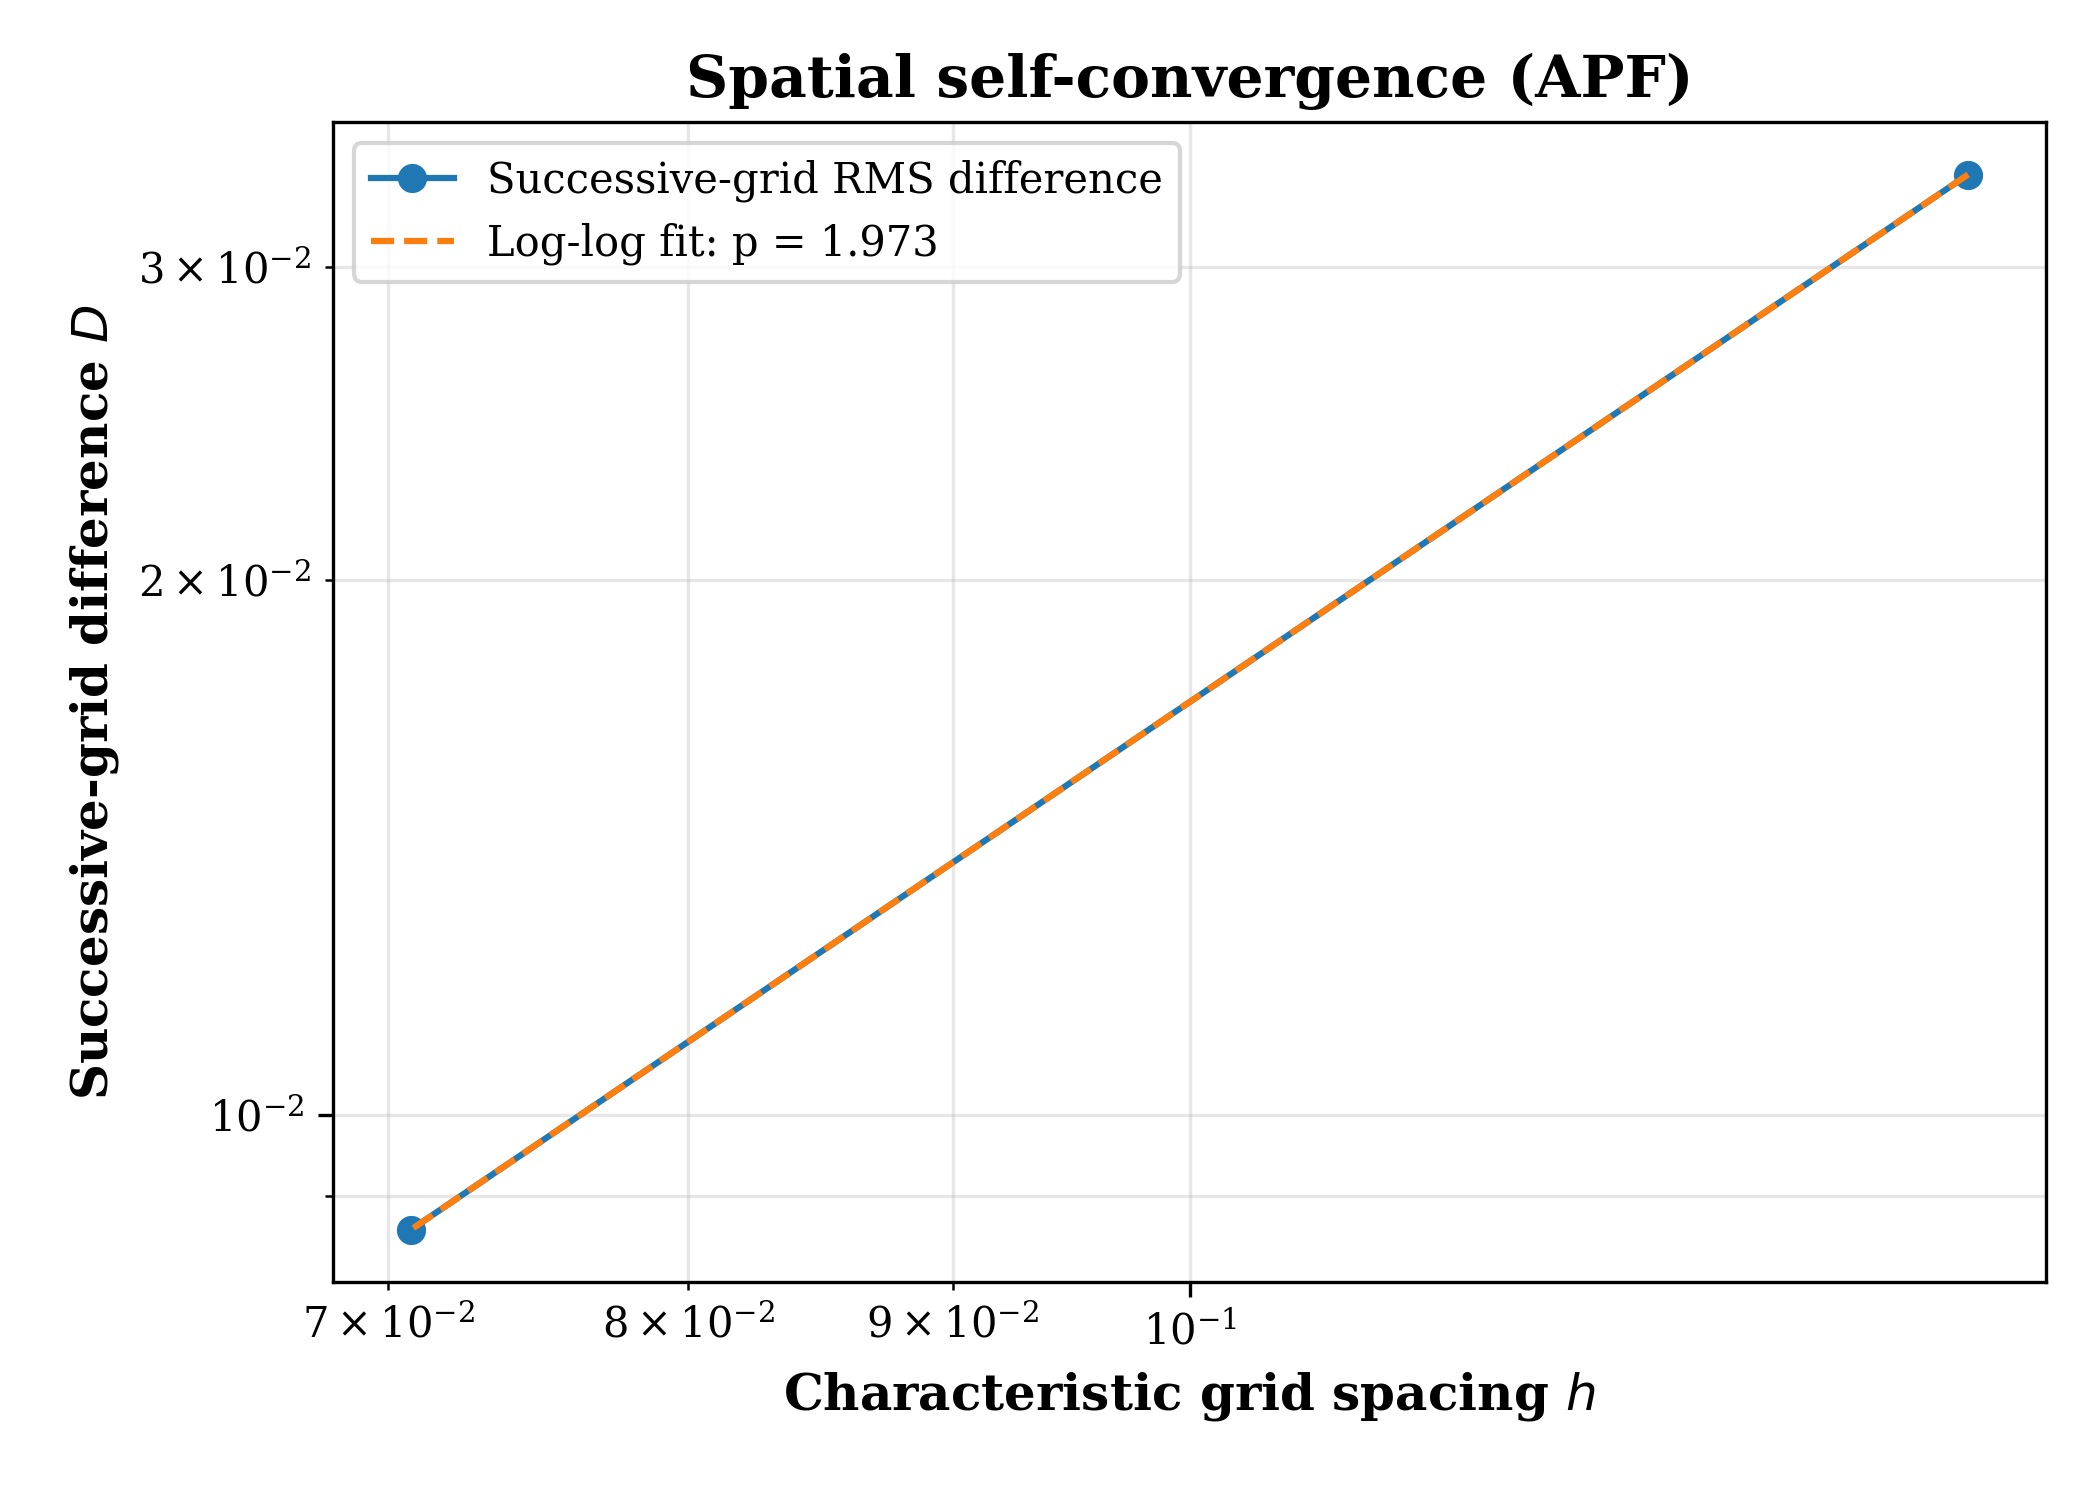
\includegraphics[width=\linewidth]
    {figures/grid_self_convergence_APF.png}

    {\small (a) APF}
\end{minipage}
\hfill
\begin{minipage}[t]{0.48\textwidth}
    \centering
    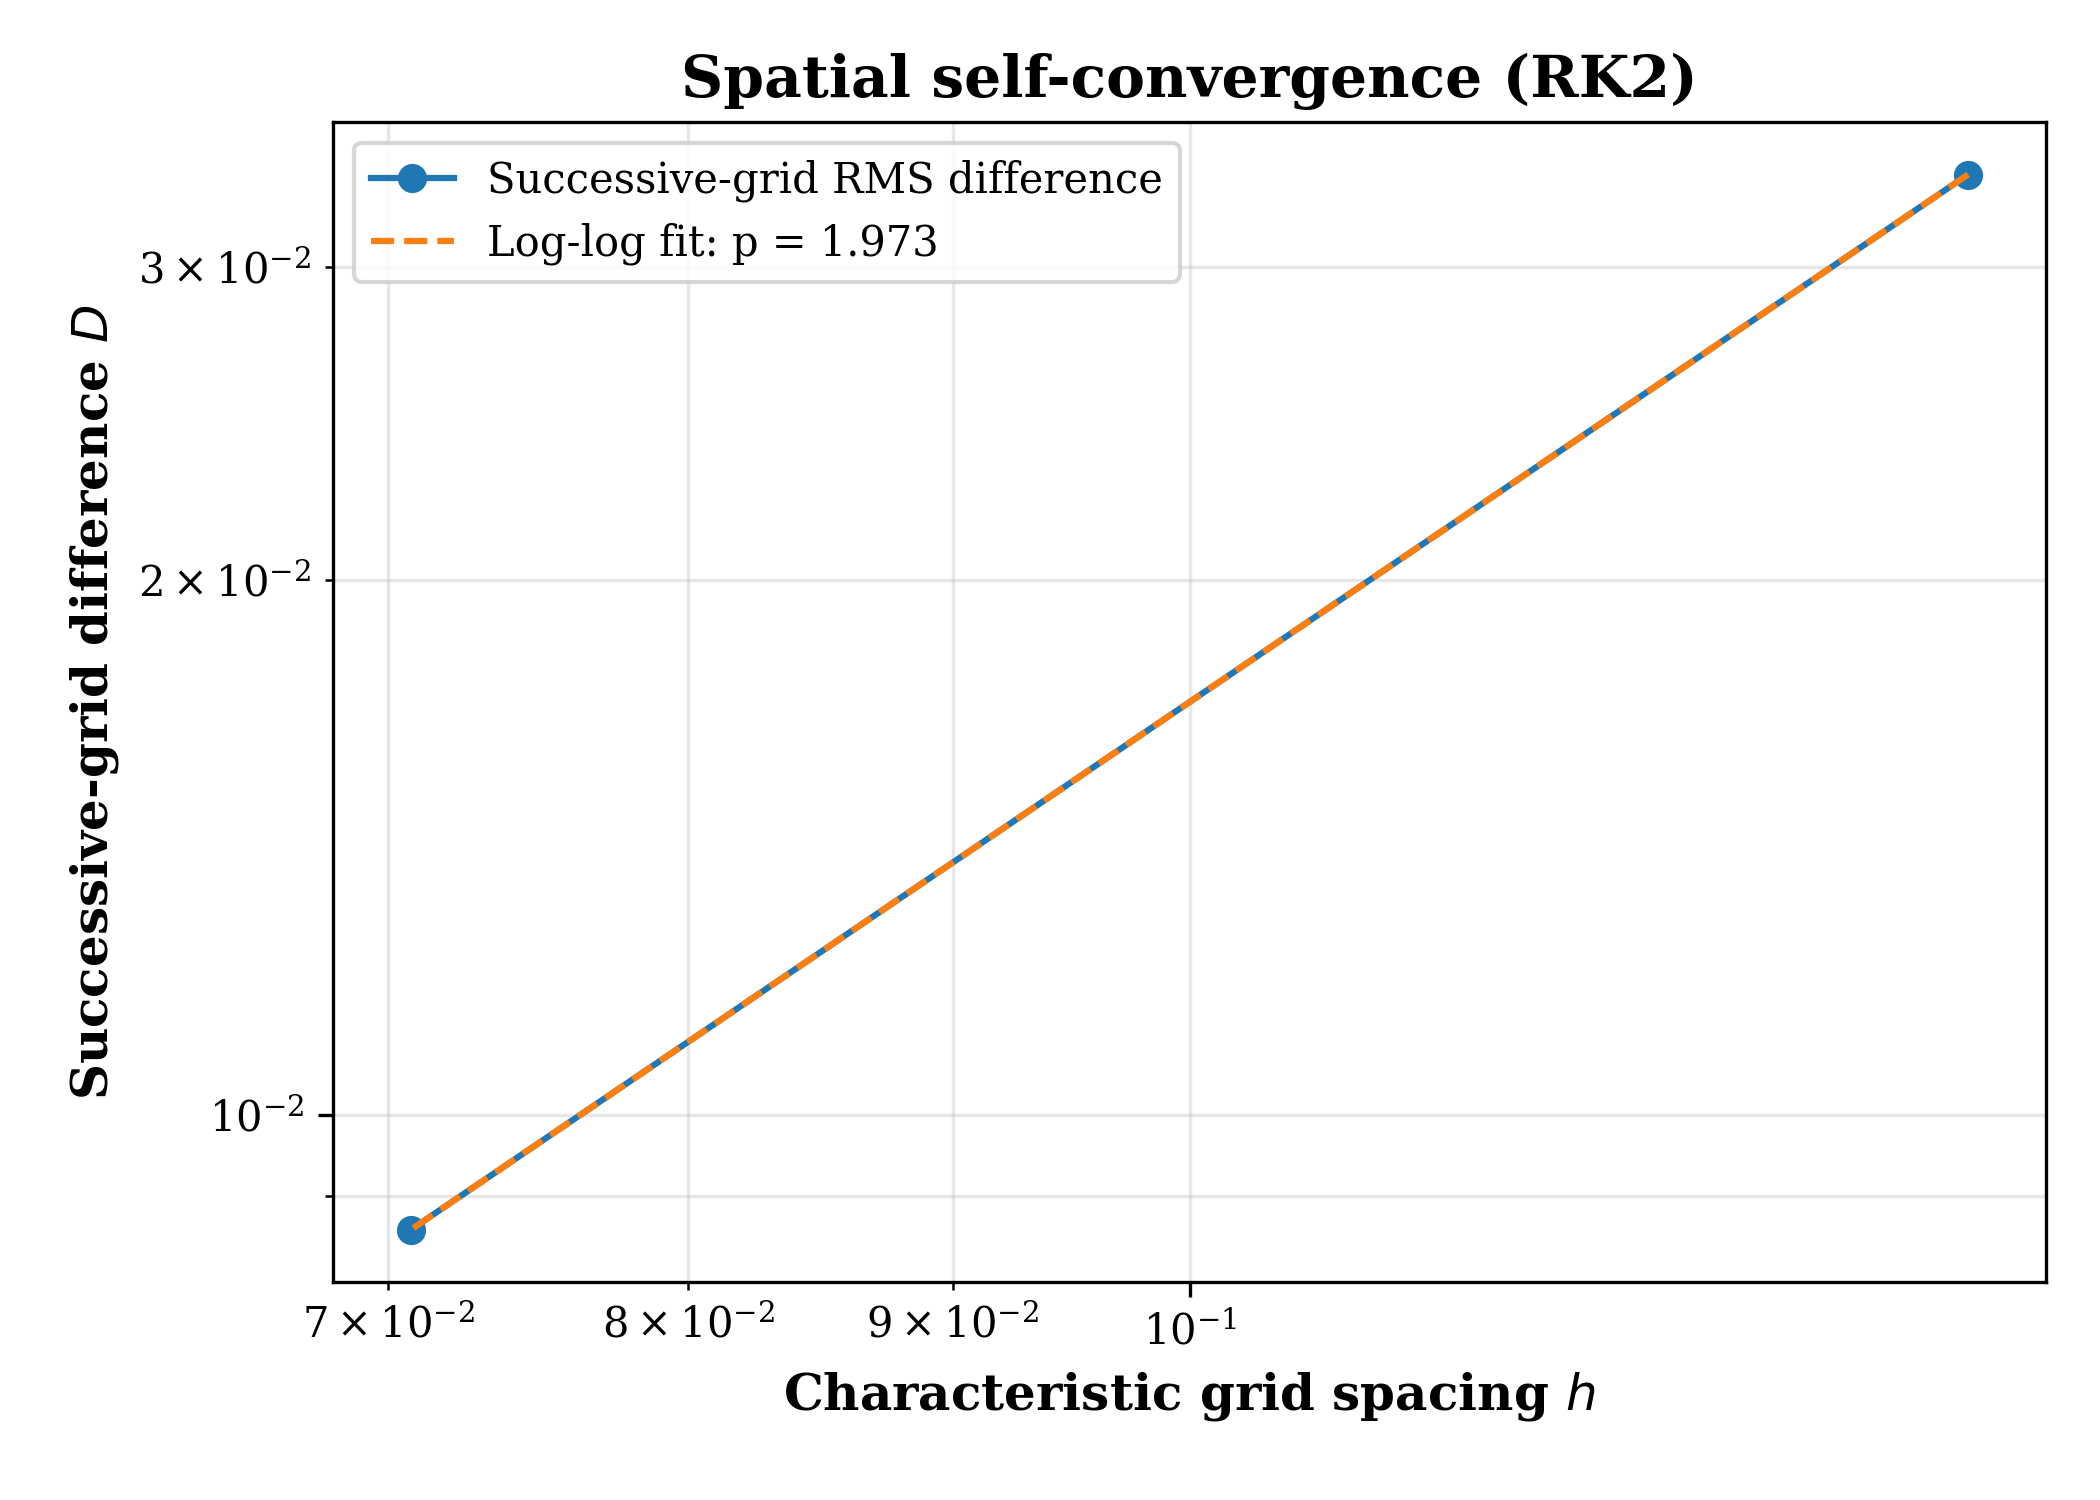
\includegraphics[width=\linewidth]
    {figures/grid_self_convergence_RK2.png}

    {\small (b) Explicit midpoint RK2}
\end{minipage}

\vspace{0.4cm}

\begin{minipage}[t]{0.48\textwidth}
    \centering
    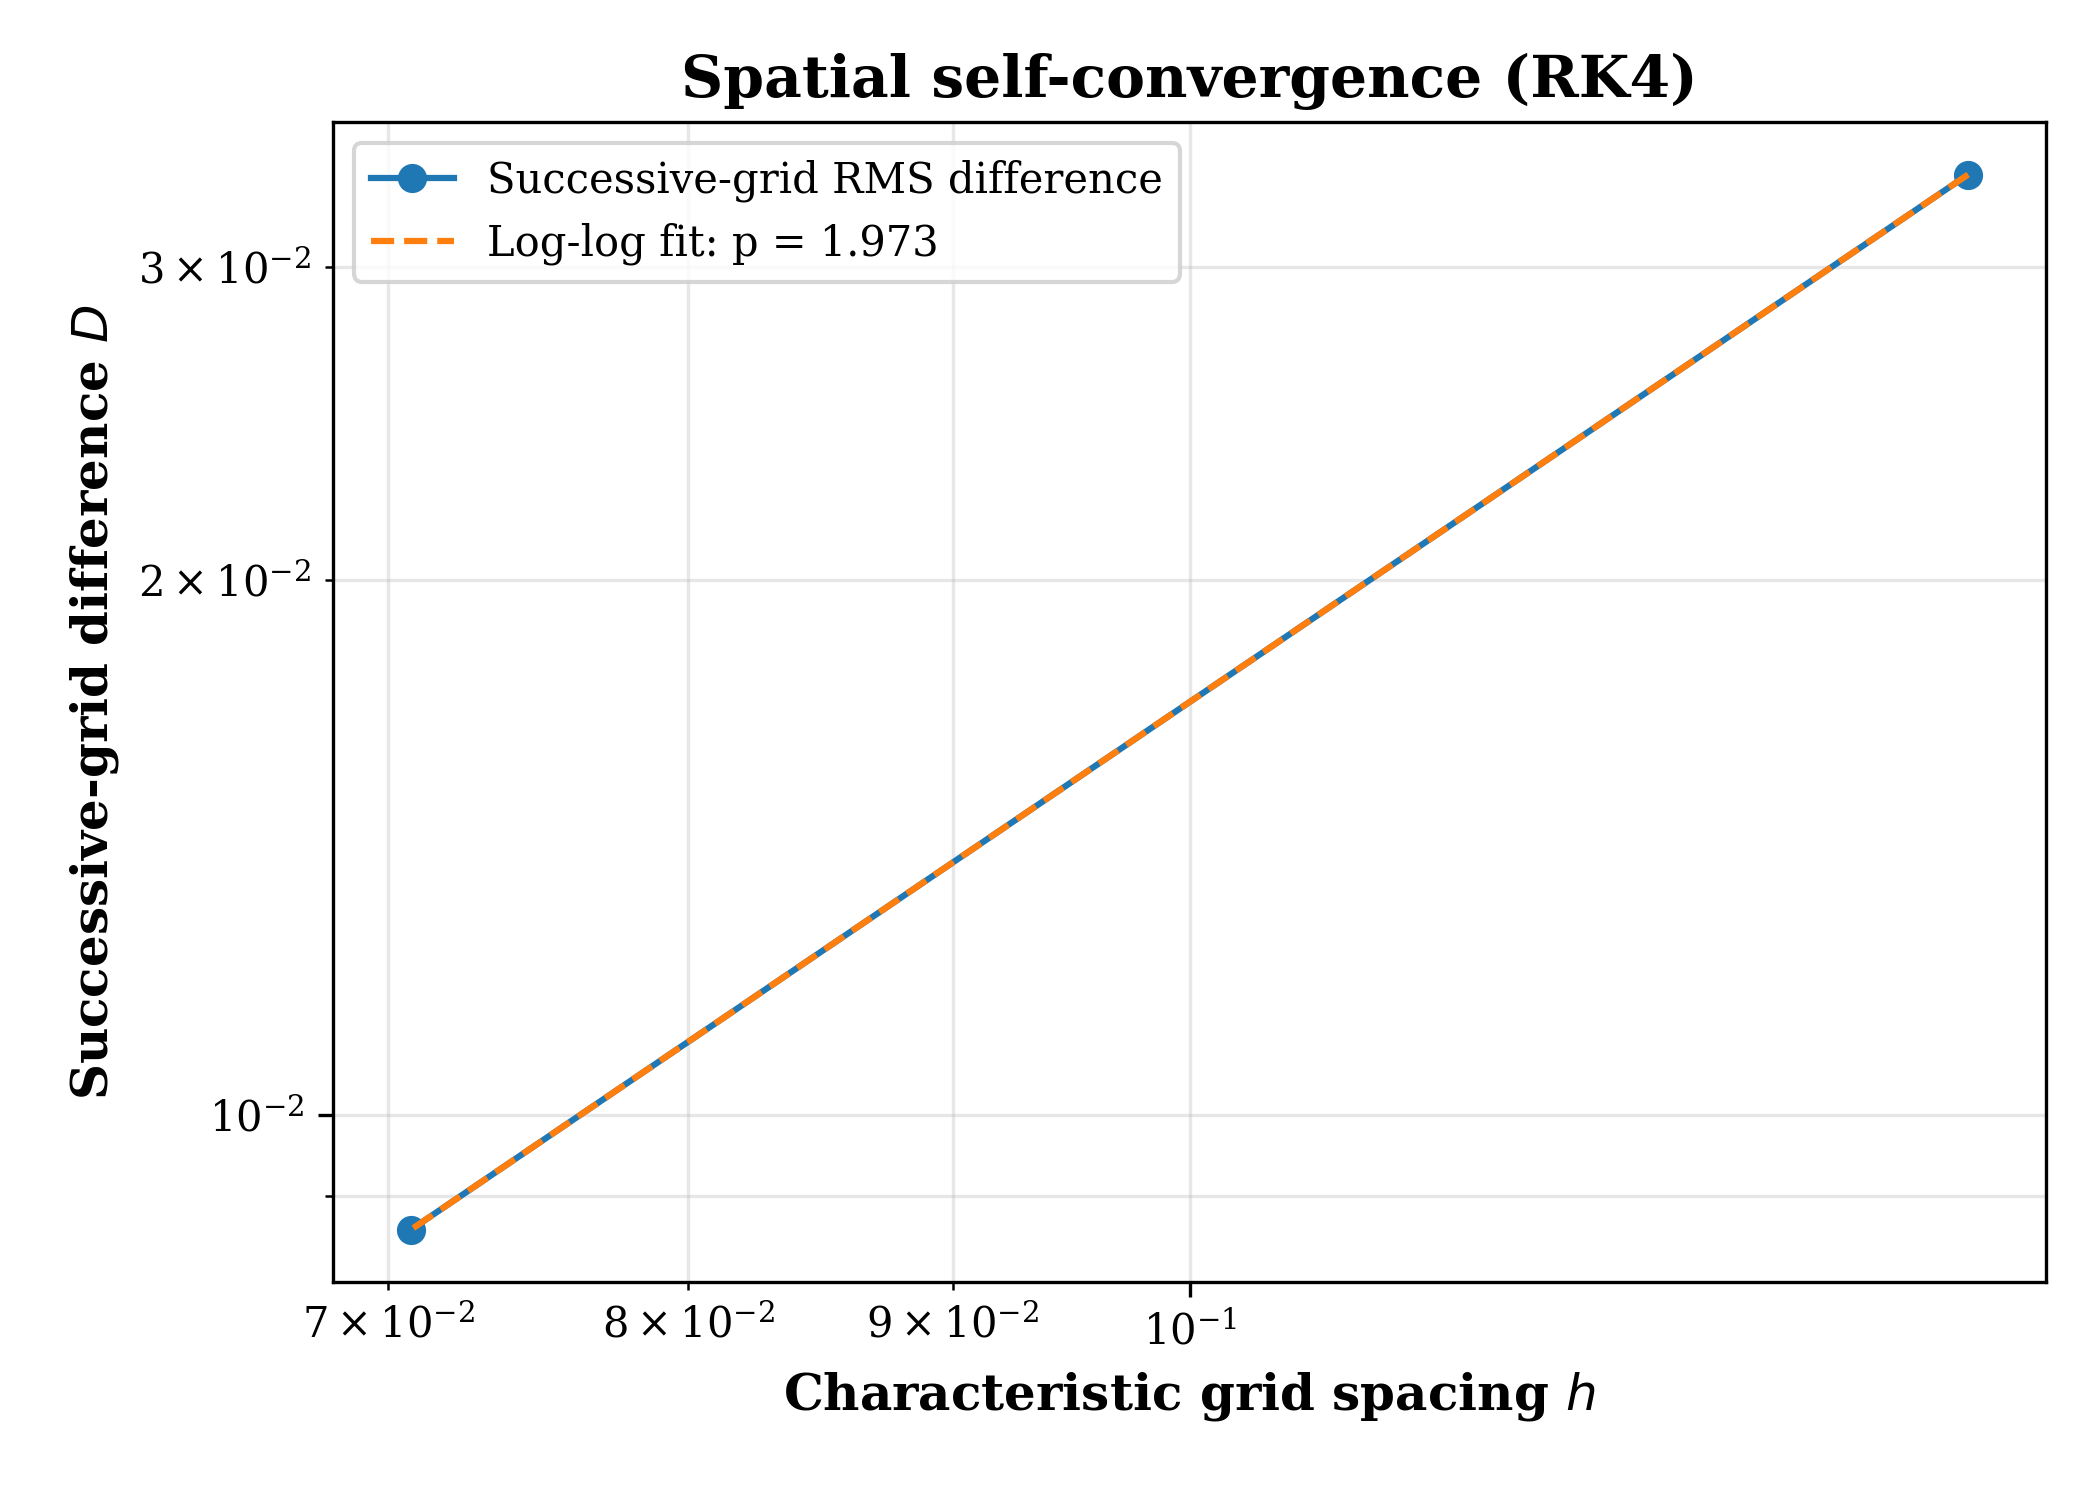
\includegraphics[width=\linewidth]
    {figures/grid_self_convergence_RK4.png}

    {\small (c) Classical RK4}
\end{minipage}
\hfill
\begin{minipage}[t]{0.48\textwidth}
    \centering
    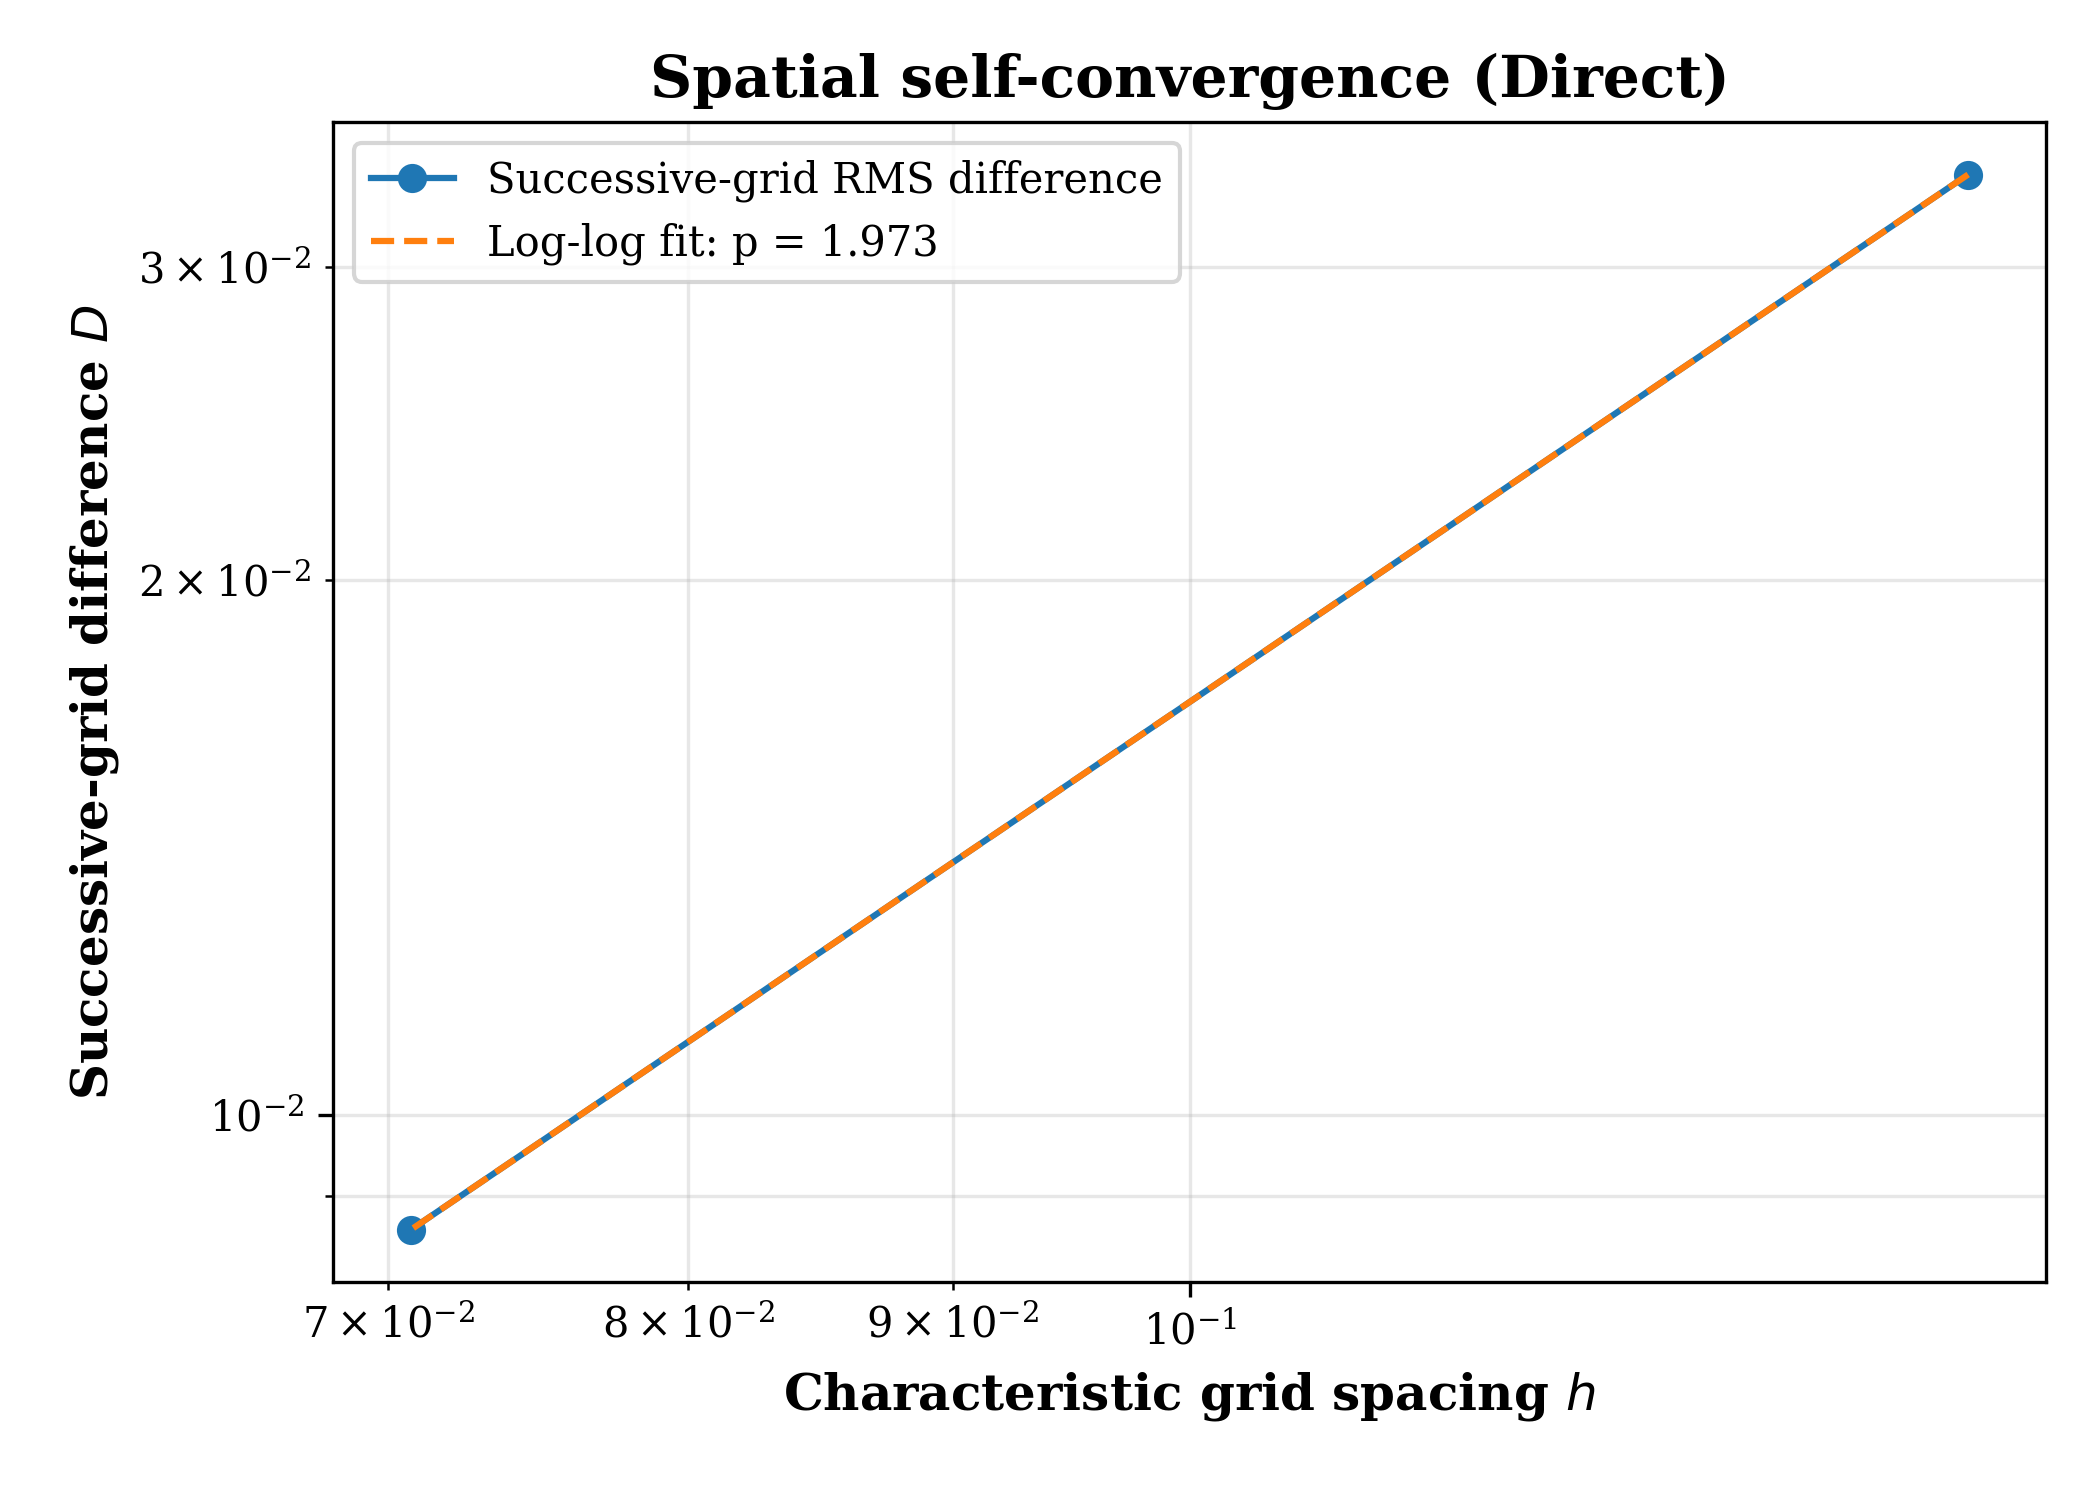
\includegraphics[width=\linewidth]
    {figures/grid_self_convergence_Direct.png}

    {\small (d) Direct implicit Euler}
\end{minipage}

\caption{Spatial self-convergence of the four numerical
methods for the linear inlet condition. Successive-grid
RMS differences are plotted against characteristic grid
spacing on logarithmic axes. All methods yield an observed
spatial convergence order of approximately two.}
\label{fig:all_solver_grid_convergence}
\end{figure}

Overall, the results demonstrate consistent second-order
spatial self-convergence across all four numerical methods.
The agreement in successive-grid differences also supports
the consistency of their implementations and their
convergence toward a common discrete steady-state solution.
However, self-convergence does not independently establish
the absolute error of the finest-grid solution.